\documentclass[a4paper,14pt]{article}
\usepackage{extsizes}
\usepackage{amsmath}
\usepackage{amssymb}
\everymath{\displaystyle}
\usepackage{geometry}
\usepackage{fancyhdr}
\usepackage{multicol}
\usepackage{graphicx}
\usepackage[brazil]{babel}
\usepackage[shortlabels]{enumitem}
\usepackage{cancel}
\columnsep=2cm
\hoffset=0cm
\textwidth=8cm
\setlength{\columnseprule}{.1pt}
\setlength{\columnsep}{2cm}
\renewcommand{\headrulewidth}{0pt}
\geometry{top=1in, bottom=1in, left=0.7in, right=0.5in}

\pagestyle{fancy}
\fancyhf{}
\fancyfoot[C]{\thepage}

\begin{document}
	
	\noindent\textbf{8FMA10, 8FMA11~-~Matemática} 
	
	\begin{center}Regra de três simples - Exercícios (Versão estudante)
	\end{center}
	
	
	\noindent\textbf{Nome:} \underline{\hspace{10cm}}
	\noindent\textbf{Data:} \underline{\hspace{4cm}}
	
	%\section*{Questões de Matemática}
	\begin{multicols}{2}
		Para os exercícios de regra de três simples serão necessárias duas igualdades. Sendo $x$ e $y$ grandezas proporcionais:
		\begin{itemize}
			\item se $x$ é diretamente proporcional a $y$, então $\frac{x_1}{y_1} = \frac{x_2}{y_2}$;
			\item se $x$ é inversamente proporcional a $y$, então $x_1 \cdot y_1 = x_2 \cdot y_2$
		\end{itemize} 
		\begin{enumerate}
	    	\item Uma pessoa ganha R\$ 280,00 em 4 dias. Qual é o salário mensal dessa pessoa? (Lembre-se para cálculos de salários, o mês é de 30 dias.) \\\\\\\\\\\\\\\\\\\\
	    	\item No início de uma viagem, Eduardo comprou meia dúzia de barras de chocolate, todas iguais e de mesmo preço totalizando R\$ 12,50. Ao fim dessa viagem, ele comprou mais barras do mesmo chocolate. Quanto ele gastou na 2ª compra? \\\\\\\\\\\\\\\\\\\\
	    	\item Um automóvel, viajando com velocidade constante, percorreu os 120 primeiros quilômetros em 1 hora e 40 minutos. Sabendo que levou 3 horas e 40 minutos para fazer o percurso total, calcule a distância total percorrida. \\\\\\\\\\\\\\\\\\
	    	\item A família Silva, viajando de automóvel, levou 3,5 horas para percorrer os 400 últimos quilômetros de uma estrada. Sabendo que o comprimento dessa estrada é de 850 quilômetros, quanto tempo os Silva levaram para percorrê-la?(Admita constante a velocidade.) \\\\\\\\\\\\\\\\
	    	\item Roberto viajou de trem para o interior e percebeu que o trem, em média, percorria 8 quilômetros a cada 6min40s. Qual é a velocidade do trem em km/h? \\\\\\\\\\\\\\\\\\\\
	    	\item Um avião, voando a 700 km/h, vai de São Paulo a Berlim em 14h30min, quanto tempo levará um avião que anda a 1000 km/h para fazer o mesmo percurso? \\\\\\\\\\\\\\\\\\\\\\
	    	\item Quatro torneiras iguais enchem, juntas, um tanque em 15 horas. Quanto tempo levarão seis torneiras iguais àquelas para, juntas, encherem o mesmo tanque? \\\\\\\\\\\\\\\\\\\\
	    	\item Em uma biblioteca, 40\% dos livros são de ficção e 23\% são de aventura. Sabendo que há 3200 livros de ficção, qual é o número de livros de aventura nessa biblioteca? \\\\\\\\\\\\\\\\\\\\
	    	\item São necessários 12 pedreiros para construir um muro de 100 m de comprimento em duas semanas. Em dois meses (8 semanas), quantos pedreiros são necessários para construir o mesmo muro? \\\\\\\\\\\\\\\\\\\\
	    	\item São necessários 12 pedreiros para construir um muro de 100 m de comprimento em duas semanas. Quanto tempo levaria esse mesmo pessoal para construir um muro de 350m? \\\\\\\\\\\\\\\\\\\\
	    	\item Dezoito pedreiros cimentam uma quadra retangular de dimensões 30m x 15 m no mesmo tempo em que x pedreiros, com mesma capacidade de trabalho, cimentam um quadrado de perímetro 60 m. Calcule $x$. \\\\\\\\\\\\\\\\\\\\
	    	\item Uma torneira enche um tanque em 3h15min. Que fração do tanque ela enche em 35 min? \\\\\\\\\\\\\\\\\\\\
	    	\item ~
	    	\begin{enumerate}[a)]
	    		\item Júlio, trabalhando 5 horas por dia, recebe R\$ 1.180,00 por mês. Quanto irá receber se passar a trabalhar 7 horas por dia? \\\\\\\\\\\\\\\\\\\\
	    		\item Agora é a sua vez. Monte um enunciado como o do item $a$ e depois resolva-o. \\\\\\\\\\\\\\
	    	\end{enumerate}
    	    \item Um caminhão tanque de 70000 L descarrega 40000 L em 25 minutos. Quanto tempo o caminhão levaria para encher um tanque de 30000 L? \\\\\\\\\\\\\\\\\\\\
    	    \item A escala de um mapa é 1 : 40000. Qual é o valor real de uma distância, em km, que nesse mapa é representado por um segmento de 7 cm? \\\\\\\\\\\\\\\\\\\\
    	    \item Uma escola será construída em um terreno com o formato de um quadrado, que tem lado igual a 3,7 cm em um mapa cuja escala é de 1 : 2000. A área desse terreno medirá, na realidade:
    	    \begin{enumerate}[a)]
    	    	\item 5476 m²
    	    	\item 6197 m²
    	    	\item 6802 m²
    	    	\item 7013 m²
    	    	\item 7400 m² \\\\\\\\\\\\\\\\\\\\
    	    \end{enumerate}
            \item Considere uma torneira que goteja 9 vezes a cada 25 segundos, Se as gotas têm sempre volume igual a 0,4 mL, qual é o volume de água que vaza por hora dessa torneira? \\\\\\\\\\\\\\\\\\\\
            \item Se uma polegada é equivalente a 2,54 cm, então $\frac{3}{4}$ de polegada, em decímetros, é equivalente a:
            \begin{enumerate}[a)]
            	\item 33,86
            	\item 0,1905
            	\item 6,4516
            	\item 19,05
            	\item 0,3386 \\
            \end{enumerate}
            \item Dois pintores, $A$ e $B$, são capazes de pintar um mesmo muro em 12 e 21 horas, respectivamente. Em cada metro quadrado, o pintor $B$ emprega 4 minutos a mais que o pintor $A$. Calcule a área do muro. \\\\\\\\\\\\\\\\\\\\
            \item Um produto é vendido em embalagens de dois tamanhos: 150 g e 85 g, representados no quadro por $X$(150) e $X$(85), respectivamente. $A$ foi o preço do produto de 150 g no fim do ano, e $B$ foi o preço do produto de 85 g no início do ano. Sabendo que $A$ e $B$ são proporcionais aos seus tamanhos, então $A$ e $B$ são, respectivamente:
            \begin{center}
            	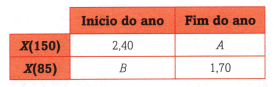
\includegraphics[width=1\linewidth]{8FMA10_imagens/adicionais-40}
            \end{center}
            \begin{enumerate}[a)]
            	\item 1,25 e 2,70
            	\item 3,10 e 1,25
            	\item 2,75 e 3,10
            	\item 1,50 e 2,80
            	\item 3,00 e 1,36 \\\\\\\\\\\\\\\\
            \end{enumerate}
        	\item O custo de fabricação de uma peça de computadores é inversamente proporcional ao número de peças fabricadas. Se o custo de fabricação de 240 peças é 310 reais, qual é o custo de fabricação de 120 peças? \\\\\\\\\\\\\\\\\\\\
        	\item João compra com toda sua mesada 50 pacotes de figurinhas. Sabendo que um pacote de figurinhas custa R\$ 2,40, quantos bonés poderá comprar com sua mesada se cada boné custar R\$ 30,00? \\\\\\\\\\\\\\\\\\\\
   	    \end{enumerate}
    \end{multicols}

\end{document}